\documentclass[twocolumn]{IEEEtran}
\usepackage{graphicx}
\usepackage[utf8x]{inputenc}
\usepackage{times}
\usepackage{amssymb,amsfonts}
\usepackage[tbtags]{amsmath}
\usepackage{cite}
\usepackage{pict2e}
\usepackage{float}
\usepackage{lscape}
\usepackage[all]{xy}
\usepackage{graphics,graphicx,color,colortbl}
\usepackage{times}
\usepackage{subfigure}
\usepackage{wrapfig}
%\usepackage{multicol}
\usepackage{cite}
\usepackage{url}
\usepackage[tbtags]{amsmath}
\usepackage{amsmath,amssymb,amsfonts,amsbsy}
\usepackage{listings}
\usepackage{bm}
\usepackage{algorithm}
\usepackage{algorithmic}
\usepackage[centerlast, small]{caption}
\usepackage[colorlinks=true, citecolor=blue, linkcolor=blue, urlcolor=blue, breaklinks=true]{hyperref}
\hyphenation{ele-men-tos he-rra-mi-en-ta cons-tru-yen trans-fe-ren-ci-a pro-pu-es-tas si-mu-lar vi-sua-li-za-cion}

\begin{document}
\title{Osciladores de anillo e Inversores NMOS y CMOS}

\author{Nicolás Arias Código: $261692$ \url{ndariass@unal.edu.co}\\
	David Ricardo Martínez Código: $261931$ \url{drmartinezhe@unal.edu.co}\\
	Oscar Rojas Código: $xxxxxx$ \url{oarojasg@unal.edu.co}\\
	Universidad Nacional de Colombia}
\markboth{Osciladores de anillo e Inversores NMOS y CMOS.}{}
\maketitle

\begin{abstract}
En la práctica de laboratorio que se describe a continuación se hizo el montaje de un un negador NMOS y uno CMOS, midiendo la respuesta en DC y los tiempos de respuesta. De igual modo, se hizo el montaje y la medición del ciclo de histéresis de un ``smith  trigger'', y por último, la implementación de dos osciladores: uno en configuración de anillo y un oscilador controlado por voltaje, de modo que es posible compararlos y determinar las ventajas y desventajas de cada uno.
\end{abstract}

\begin{keywords}
Negador CMOS, Negador NMOS, Oscilador, Smith trigger.
\end{keywords}

\section{Introducción}
\subsection{Cálculo del parámetro $k_n$}
A partir de la medición de la función de transferencia del circuito de la fig~\ref{introf1}  es posible determinar el parámetro $k_n$.

\begin{figure*}[H]%[!t]
\centering
	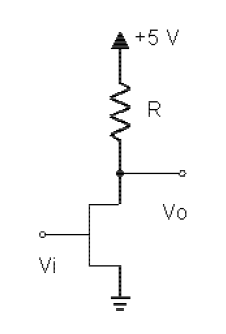
\includegraphics[width=0.40\textwidth]{pics/intro1.png}
	\caption{Negador NMOS a partir del cual se calcula el parámetro $k_n$ del transistor.}
	
	\label{introf1}

\end{figure*}

Dadas las ecuaciones de corriente de drain para región de saturación~\ref{eq1p1} y triodo~\ref{eq1p2}

\begin{equation}
I_D = k_n(V_{GS}-V_T)^2
\label{eq1p1}
\end{equation}

\begin{equation}
I_D = 2k_n[(V_{GS}-V_T)V_{DS}-V_{DS}^2]
\label{eq1p2}
\end{equation}

es posible despejar $k_n$ para varias parejas $V_{GS}$, $V_{DS}$ medidas. La corriente también se puede expresar como una función lineal de $V_{DS}$ 

\begin{equation}
I_D = \dfrac{V_{DD}-V_{DS}}{R}
\end{equation}

\section{Medidas de características DC de inversores NMOS}
En la tabla~\ref{t1p1} se observan los valores de $k_n$ medidos para diferentes pares de valores $V_{in}$, $V_{out}$. Naturalemente, para cada punto se usa una relación diferente de $k_n$ considerando si para dicho par de puntos el transistor se encuentra en región de triodo o de saturación. Para cada valor de  $R_D$ se escogieron 3 puntos. Finalmente, se halla el promedio de los valores calculados, así como una desviación estándar de los datos. Llama la atención que el valor de $V_T$ presenta una ligera variación. Para $R_D=1$ k$\Omega$ se tiene $V_T=2$ V. Para los otros valores de resistencia se tiene  $V_T=1.8$ k$\Omega$

\begin{table}[h]
	%% increase table row spacing, adjust to taste
	\renewcommand{\arraystretch}{1.1}
	% if using array.sty, it might be a good idea to tweak the value of
	 %\extrarowheight as needed to properly center the text within the cells
	\caption{Valor de $k_n$ del transistor usado a partir de diferentes parejas de puntos $V_{in}$, $V_{o}$}
	\label{t1p1}
	\centering
	%% Some packages, such as MDW tools, offer better commands for making tables
	%% than the plain LaTeX2e tabular which is used here.
	\begin{tabular}{|c|c|c|}
	\hline
	\bf $V_{GS}$ (V) & \bf $V_{DS}$ (V) & \bf $k_n$ (mA/V$^2$) \\
	\hline
	3.6 & 5.0 & 0.391	\\ \hline 
	4.5 & 4.0 & 0.320	\\ \hline
	5.3 & 3.0 & 0.278	\\ \hline \hline
	2.5 & 4.5 & 0.651	\\ \hline
	2.7 & 3.0 & 0.788   \\ \hline
	3.1 & 1.0 & 0.665   \\\hline \hline
	3.0 & 4.0 & 0.139   \\ \hline
	3.3 & 3.0 & 0.133   \\\hline
	3.8 & 1.0 & 0.167   \\ \hline \hline
	    & \ \ \ \ \ \  Promedio  & 	0.392	\\ \hline 
		& Desv. estándar & 0.250	\\ \hline 
	
	\end{tabular}
\end{table}

En la figura~\ref{p1ff22} se muestra un ejemplo de la medición hecha de $V_{out}$ vs $V_{in}$. En este caso es la medida para $R_D=4.7$ k$\Omega$.



\begin{figure*}[H]%[!t]
\centering
	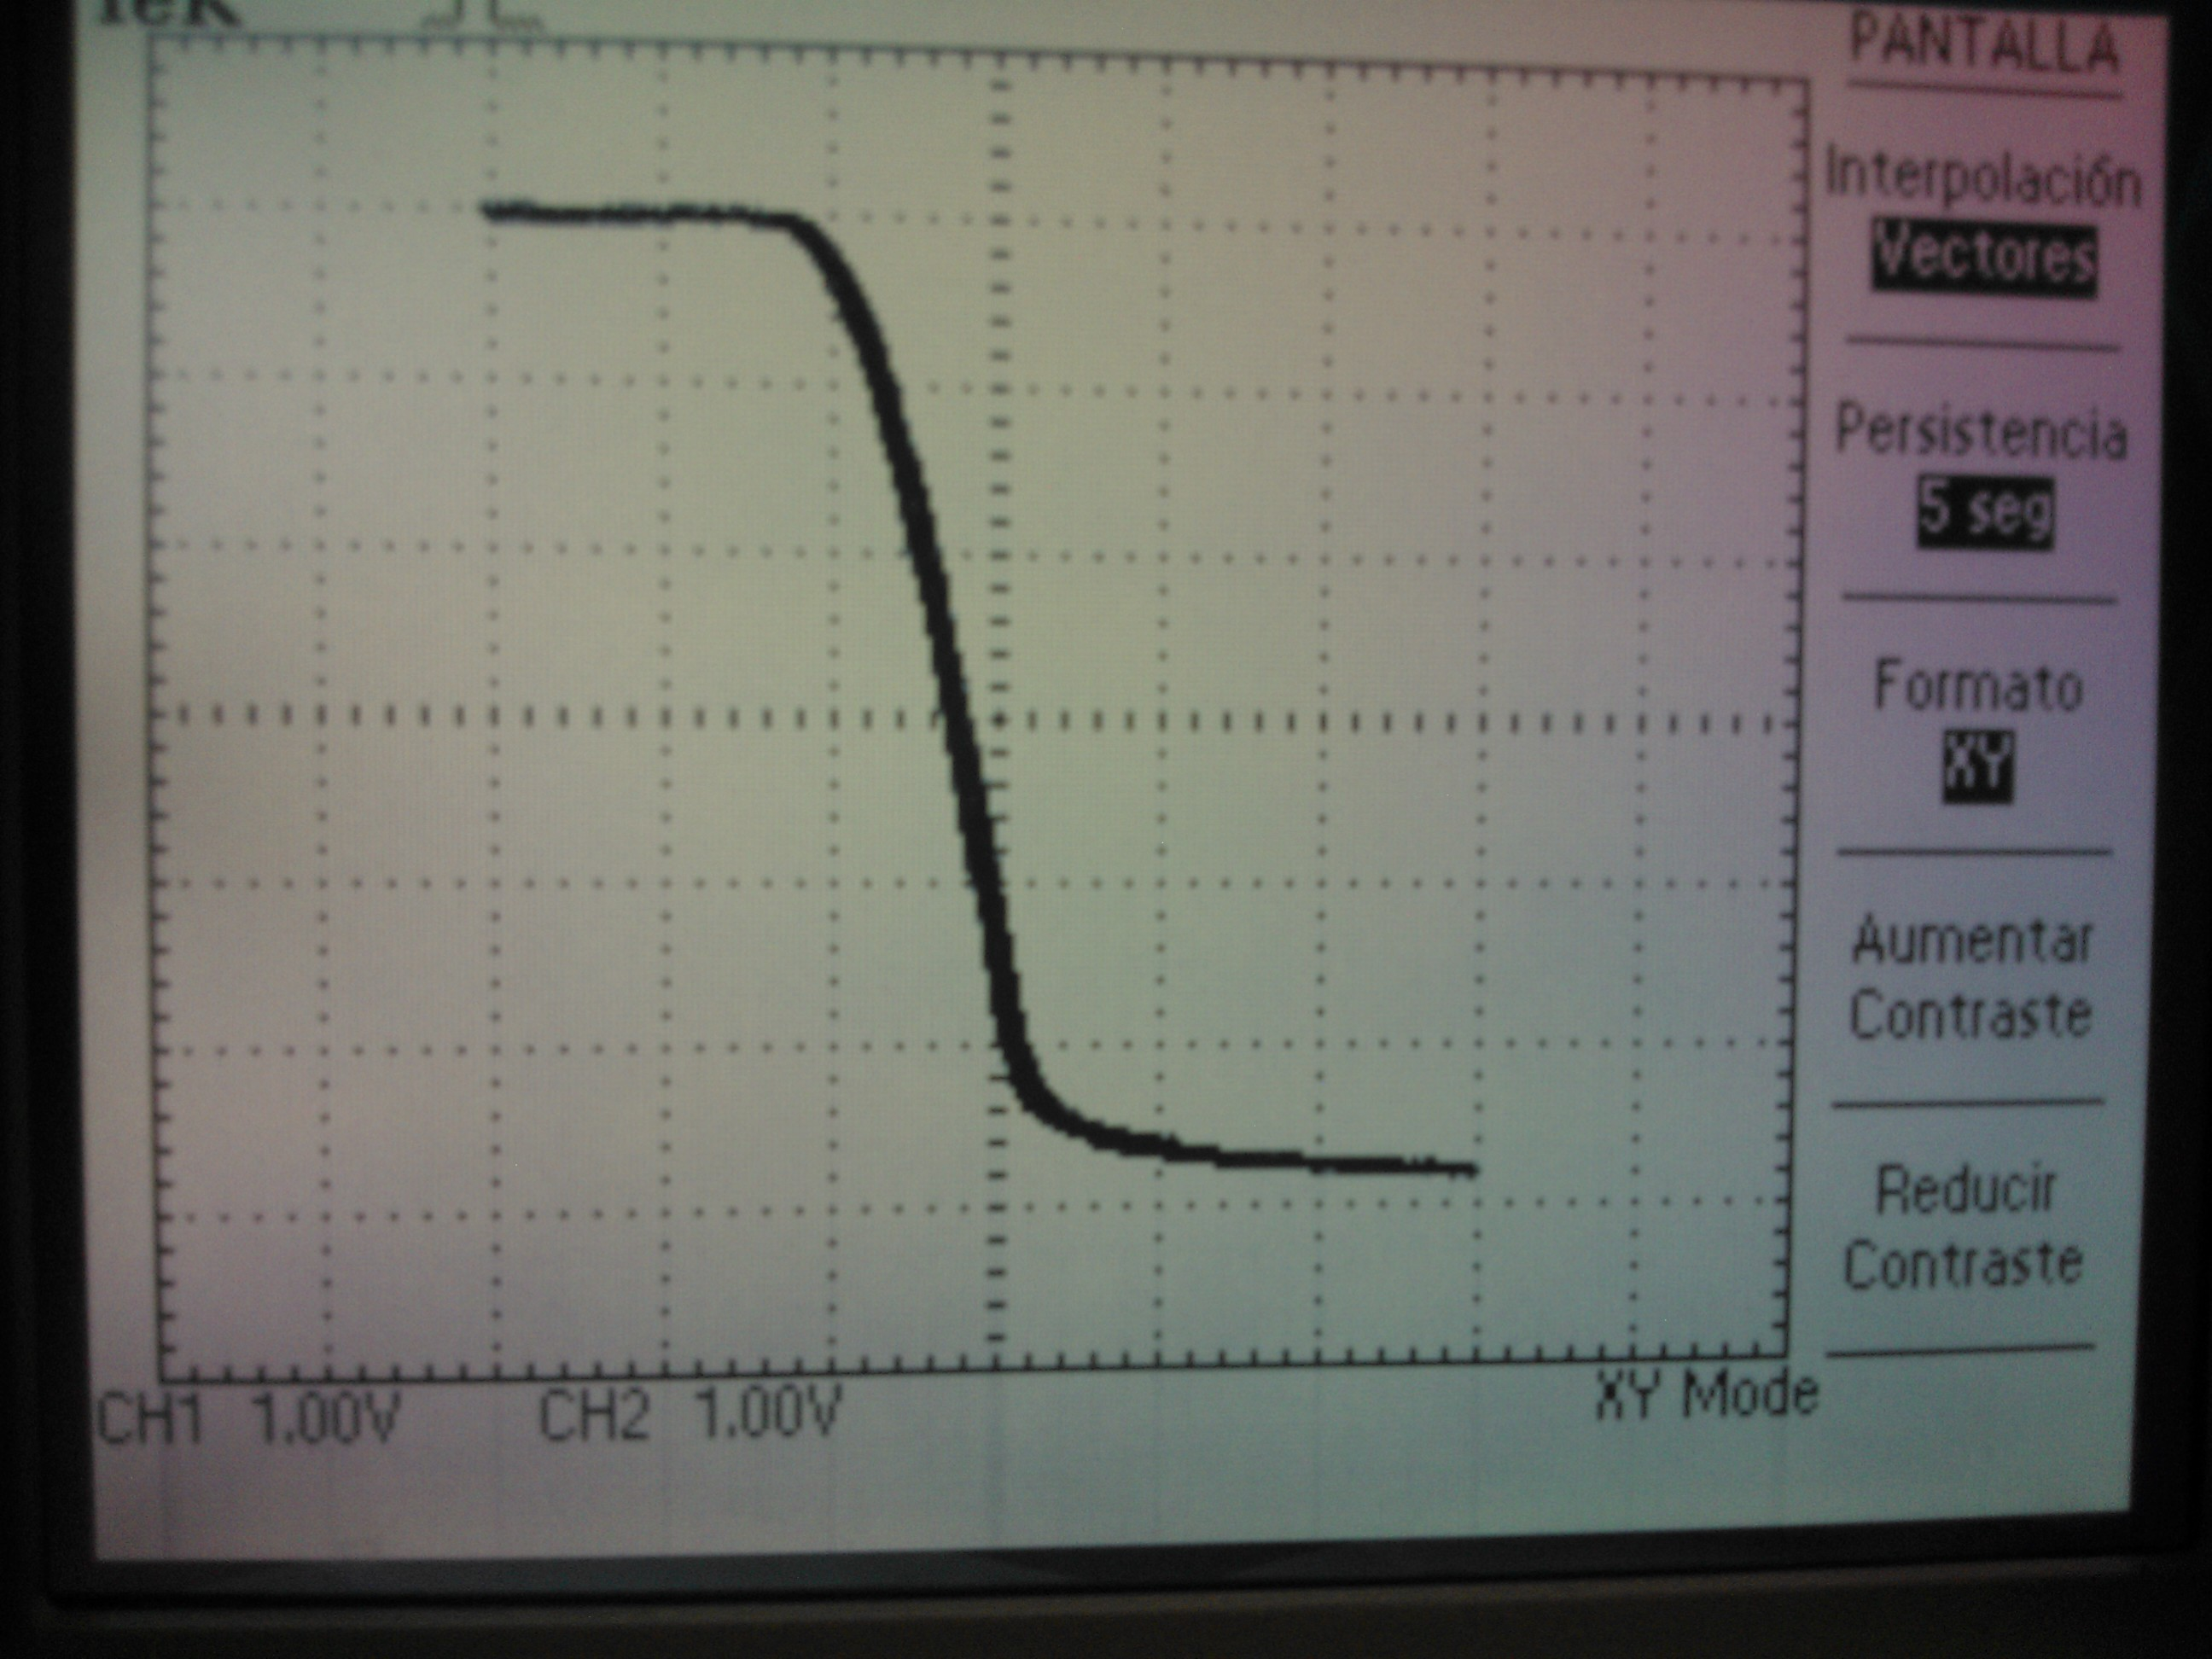
\includegraphics[width=0.40\textwidth]{pics/WP_000070.jpg}
	\caption{$V_{out}$ vs $V_{in}$ para el negador NMOS con $R_D=4.7$ k$\Omega$}
	
	\label{p1ff22}

\end{figure*}


\section{Medidas de velocidad de respuesta de un inversor CMOS}


\section{Disparador de Schmitt trigger}


\section{Osciladores}

\subsection{Oscilador de anillo.}
Se hizo el montaje de osciladores de anillo usando 3, 5 y 7 negadores del integrado CD4069.
En las tablas~\ref{p4t1},~\ref{p4t2}~y~\ref{p4t3} se muestra la ganancia y el retraso en cada etapa (salida de cada negador de la configuración) para las configuraciones con 3, 5 y 7 negadores, respectivamente. Dichos parámetros se dan respecto a la salida $V_o$ de las configuraciones.

\begin{figure*}[H]%[!t]
\centering
	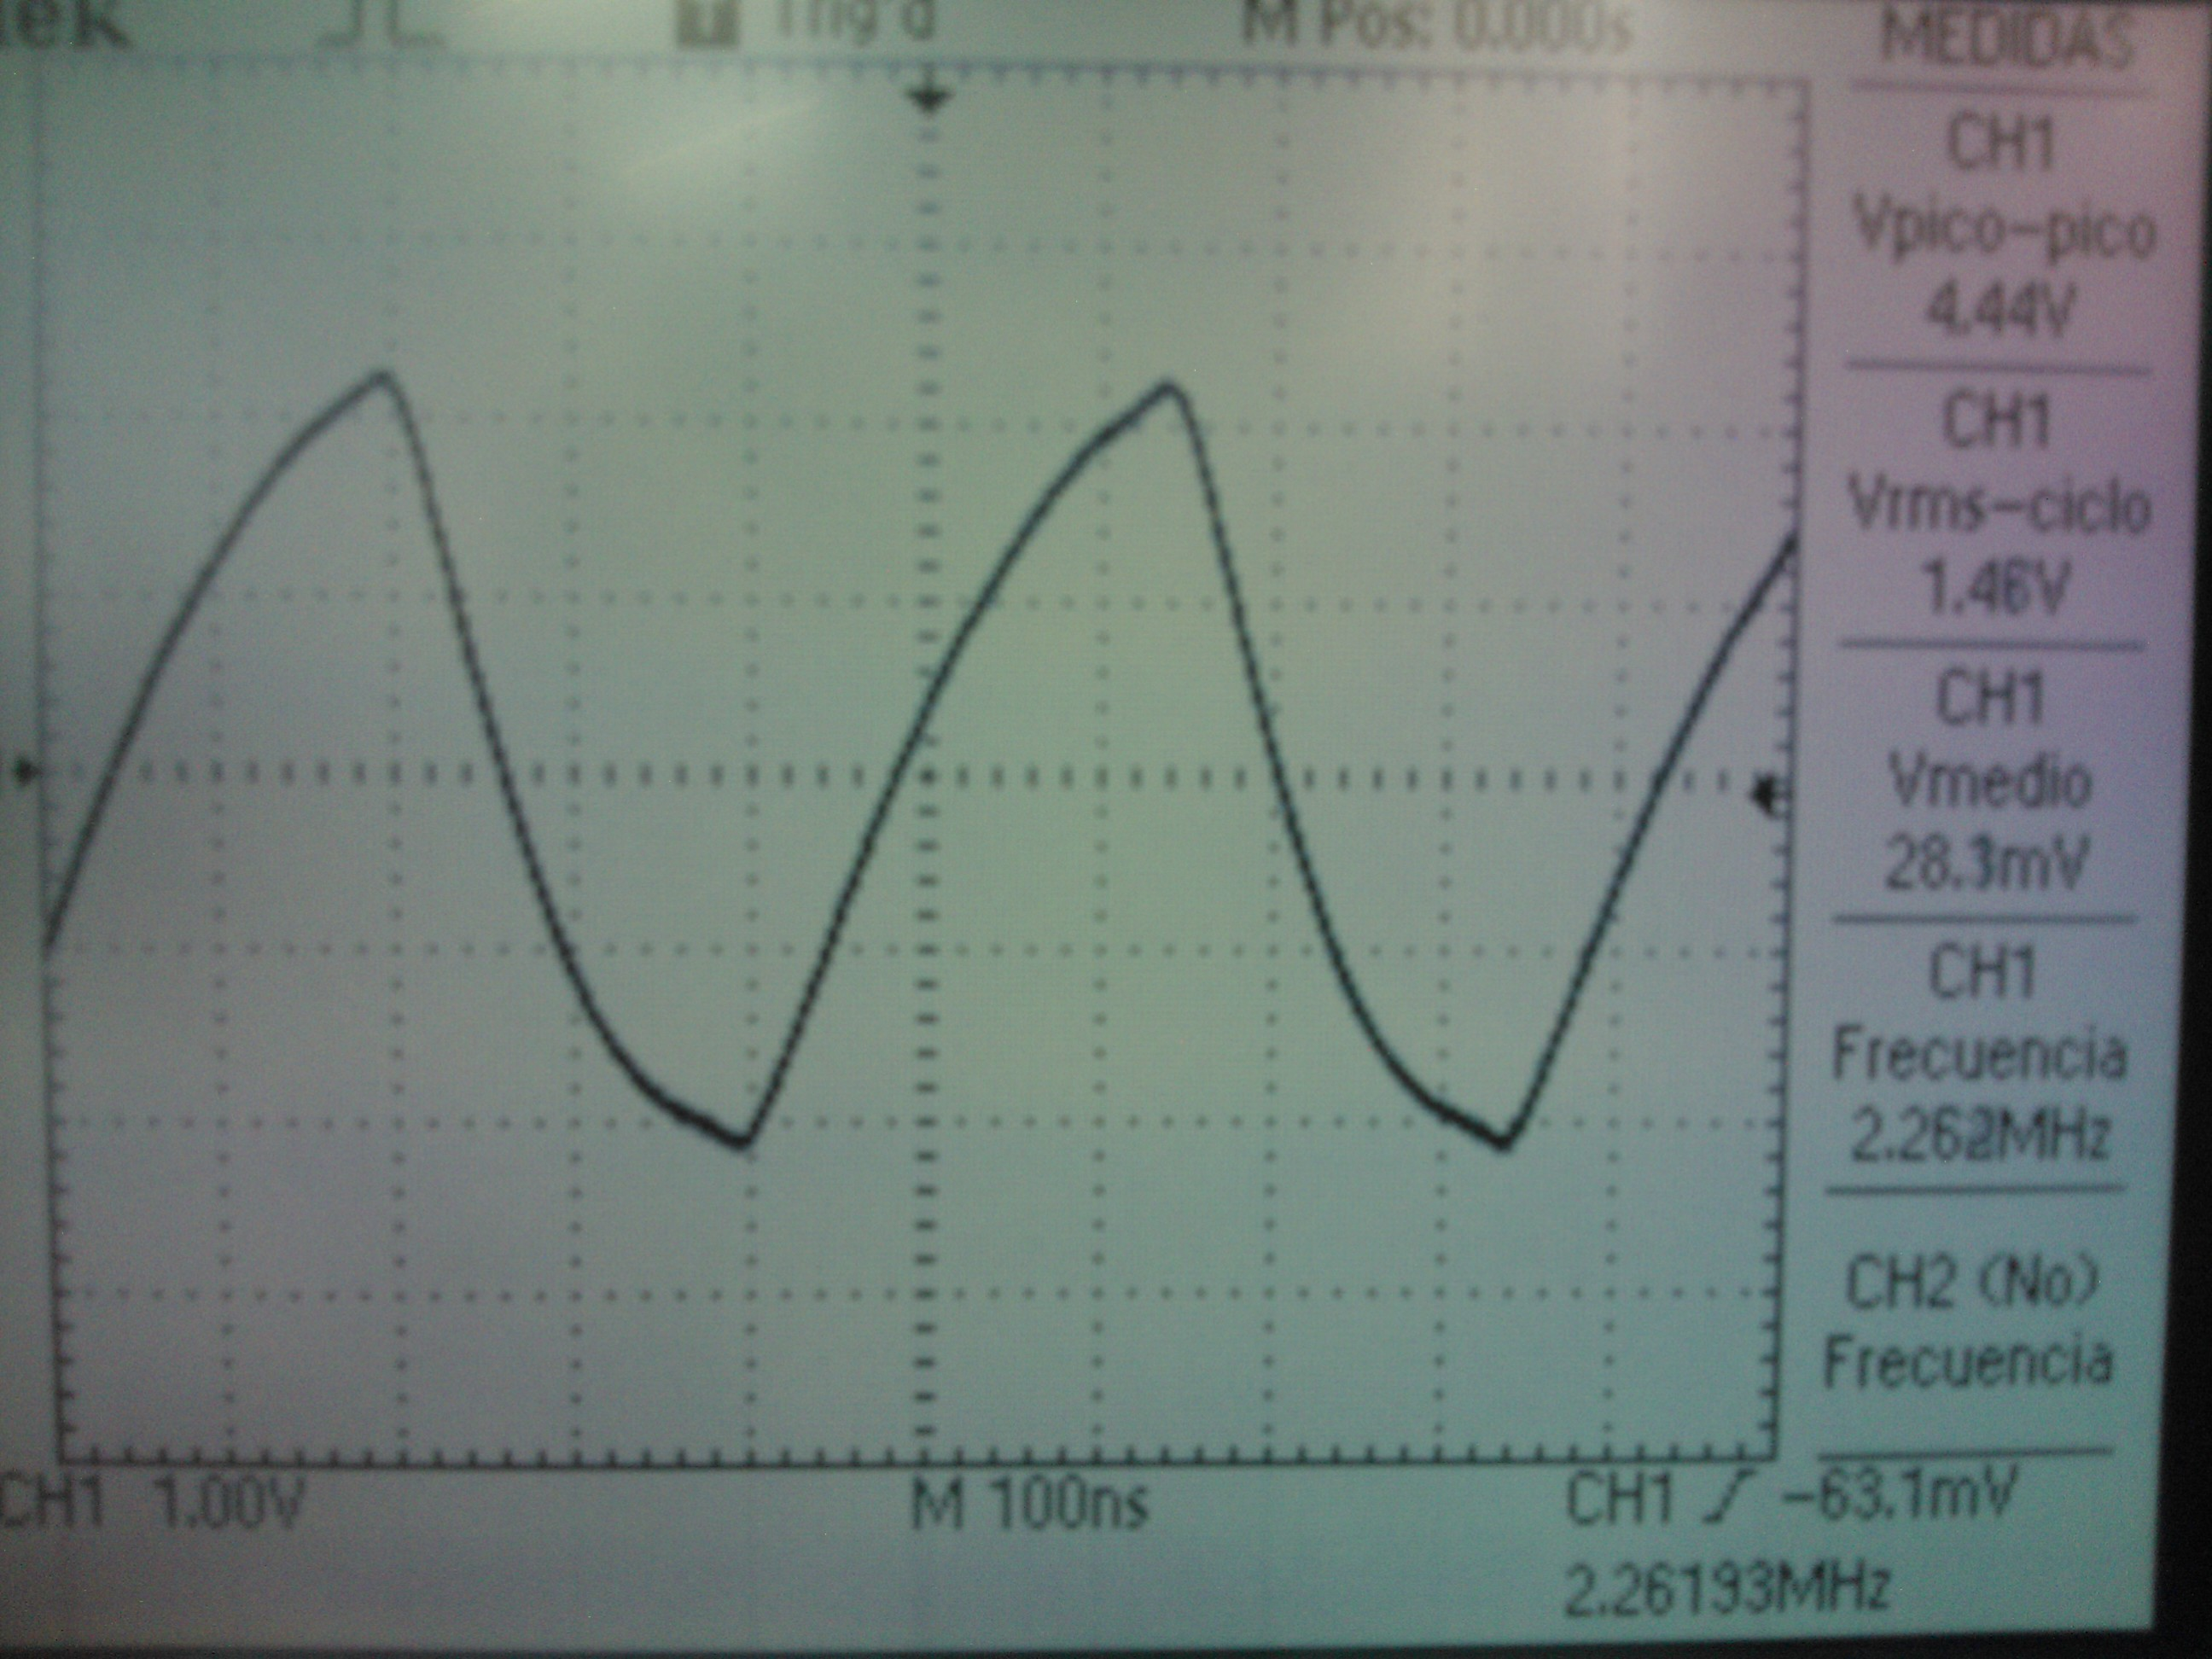
\includegraphics[width=0.40\textwidth]{WP_000051.jpg}
	\caption{Señal de salida para el oscilador en anillo con 7 negadores.}
	
	\label{anillo1}

\end{figure*}

\begin{table}[h]
	%% increase table row spacing, adjust to taste
	\renewcommand{\arraystretch}{1.1}
	% if using array.sty, it might be a good idea to tweak the value of
	 %\extrarowheight as needed to properly center the text within the cells
	\caption{Gananacia y retraso  por etapa del oscilador en anillo con 3 negadores.}
	\label{p4t1}
	\centering
	%% Some packages, such as MDW tools, offer better commands for making tables
	%% than the plain LaTeX2e tabular which is used here.
	\begin{tabular}{|c|c|c|}
	\hline
	\bf Etapa & \bf Ganancia & \bf Retraso (ns) \\
	\hline
	1 & 0.816 & 52 \\
	\hline
	2 & 0.659 & 120 \\
	\hline
	\end{tabular}
\end{table}

\begin{table}[h]
	%% increase table row spacing, adjust to taste
	\renewcommand{\arraystretch}{1.1}
	% if using array.sty, it might be a good idea to tweak the value of
	 %\extrarowheight as needed to properly center the text within the cells
	\caption{Gananacia y retraso  por etapa del oscilador en anillo con 5 negadores.}
	\label{p4t2}
	\centering
	%% Some packages, such as MDW tools, offer better commands for making tables
	%% than the plain LaTeX2e tabular which is used here.
	\begin{tabular}{|c|c|c|}%{m{2cm}m{2cm}m{2cm}}
	\hline
	\bf Etapa & \bf Ganancia & \bf Retraso (ns) \\
	\hline
	1 & 0.923 & 48 \\
	\hline
	2 & 0.989 & 100 \\
	\hline
	3 & 1.023 & 106 \\
	\hline
	4 & 1.125 & 184 \\
	\hline
	\end{tabular}
\end{table}

\begin{table}[H]
	%% increase table row spacing, adjust to taste
	\renewcommand{\arraystretch}{1.1}
	% if using array.sty, it might be a good idea to tweak the value of
	 %\extrarowheight as needed to properly center the text within the cells
	\caption{Ganancia y retraso  por etapa del oscilador en anillo con 7 negadores.}
	\label{p4t3}
	\centering
	%% Some packages, such as MDW tools, offer better commands for making tables
	%% than the plain LaTeX2e tabular which is used here.
	\begin{tabular}{|c|c|c|}
	\hline
	\bf Etapa & \bf Ganancia & \bf Retraso (ns) \\
	\hline
	1 & 0.958 & 48 \\
	\hline
	2 & 0.969 & 96 \\
	\hline
	3 & 0.969 & 136\\
	\hline
	4 & 1.043 & 156 \\
	\hline
	5 & 1.021 & 200 \\
	\hline
	6 & 1.011 & 252 \\
	\hline
	\end{tabular}
\end{table}

Se hizo de igual modo una medida más detallada de los parámetros de tiempo usando la configuración de tres negadores. Es decir, la medida corresponde a los tiempos de dos negadores en cascada. A continuación se muestra la estimación de los parámetros obtenida para cada negador.

\begin{itemize}
	\item Tiempo de almacenamiento $t_s$ = 39.5 ns 
	\item Tiempo de retraso $t_d$ = 32.0 ns
	\item Tiempo de bajada $t_f$ = 132.0 ns
	\item Tiempo de subida $t_r$ = 124 ns	
\end{itemize}

En la figura~\ref{anillo1} se muestra la tensión de salida para la configuración de 7 negadores. 

\begin{figure*}[H]%[!t]
\centering
	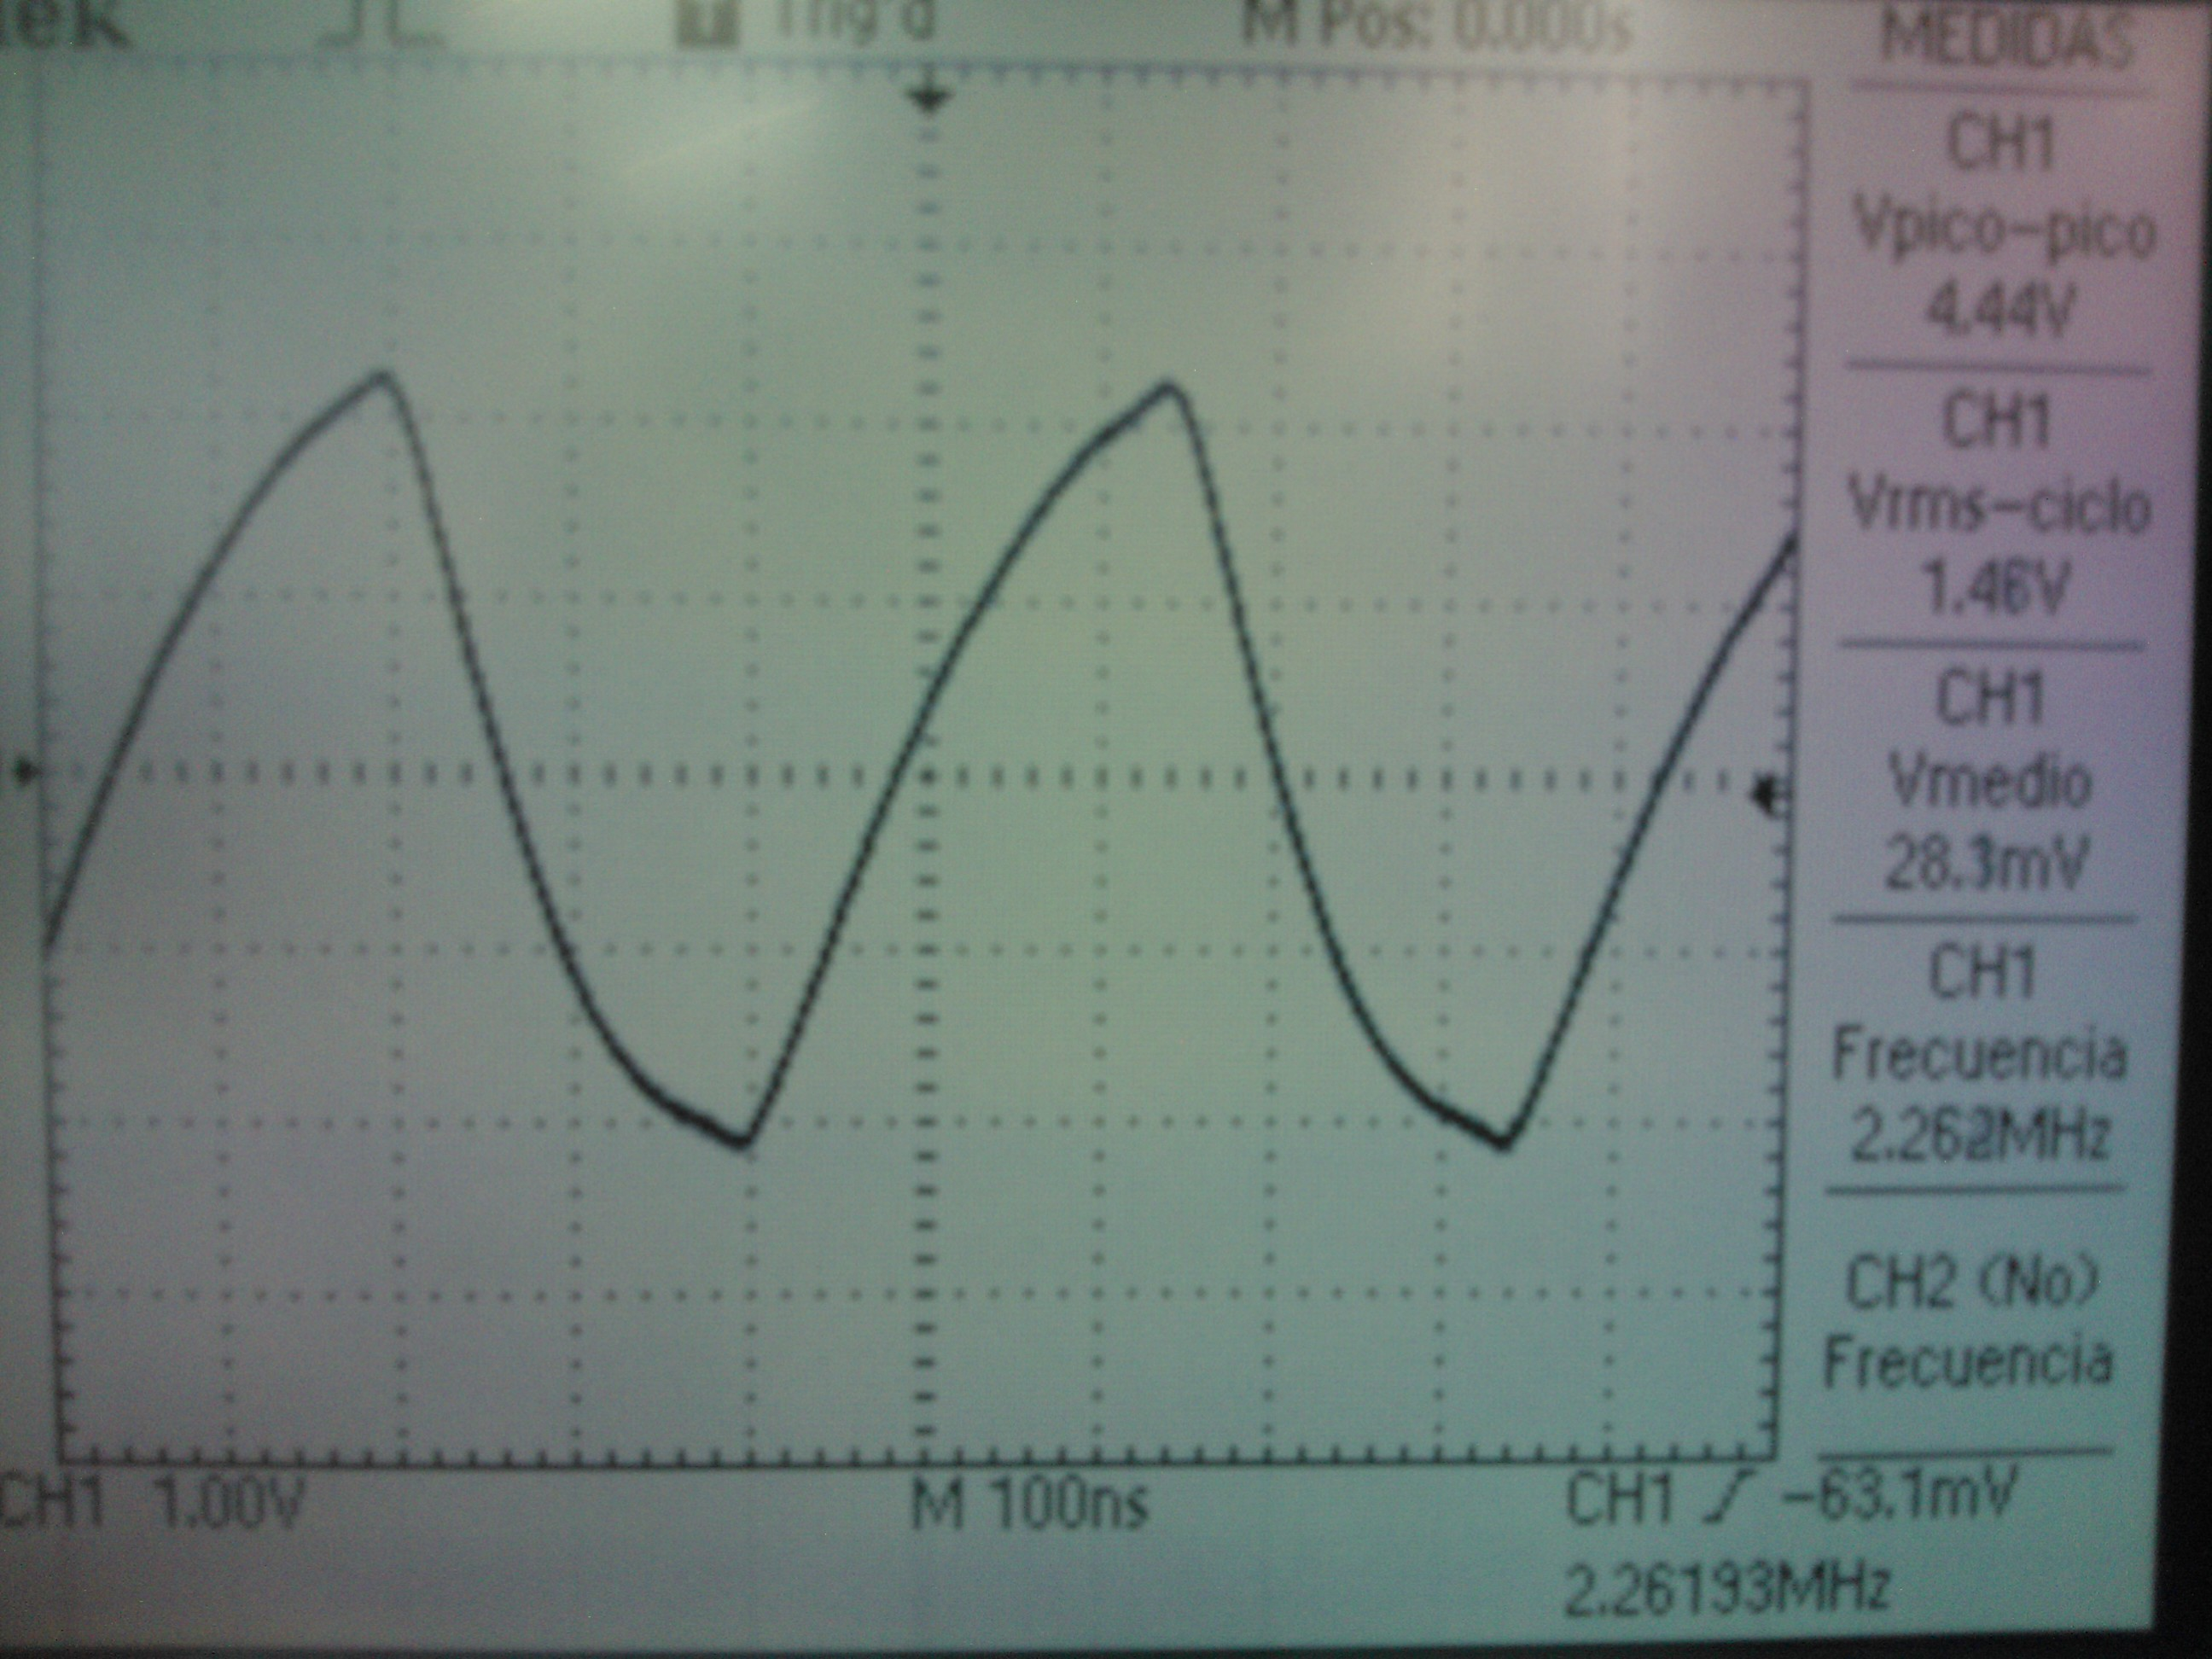
\includegraphics[width=0.40\textwidth]{WP_000051.jpg}
	\caption{Señal de salida para el oscilador en anillo con 7 negadores.}
	
	\label{anillo1}

\end{figure*}

\subsection{Oscilador controlado por voltaje.}
La configuración se probó para dos combinaciones diferentes de $R_1$ y $C_x$, en ambos casos con $V_{DD}=5$ V.

\begin{itemize}
	%%%OJO, INFORMACIÓN POR COMPLETAR
	\item $R_1$ = 10 k$\Omega$ y $C_x$ = 1 nF. En este caso se tuvo $f_{min}=36.49$ kHz y $f_{max}=68.26$ kHz (ver figura~\ref{vco_1}).
	\item $R_1=$4.7 k$\Omega$ y $C_x=$10 nF. En este caso se tuvo $f_{min}=$6.21 kHz y $f_{max}=$7.73 kHz (ver figura~\ref{vco_2}).
\end{itemize}

En ambos casos se obtuvo una señal de salida más ``limpia'' para la frecuencia inferior de cada rango, es decir cuando en el transistor $V_{GS}<V_T$

%%%el el otro grafico f vs. VA lleva este label
% \label{vco_1}

\begin{figure*}[H]%[!t]
\centering
	%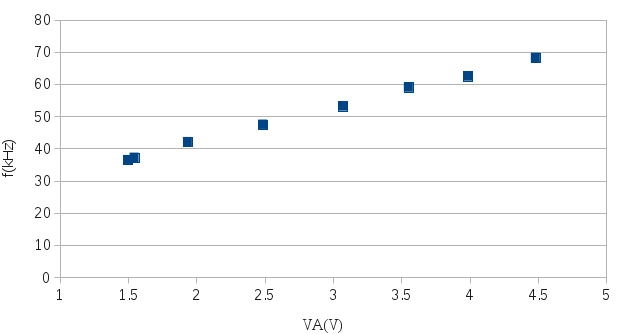
\includegraphics[width=0.45\textwidth]{./pics/vco_1.png}
	\caption{ Gráfica de frecuencia de salida $f$ vs. tensión de entrada $V_A$ para $R_1$=10 k$\Omega$ y $C_x$=1 nF.}
	
	\label{vco_1}

\end{figure*}

\begin{figure*}[H]%[!t]
\centering
	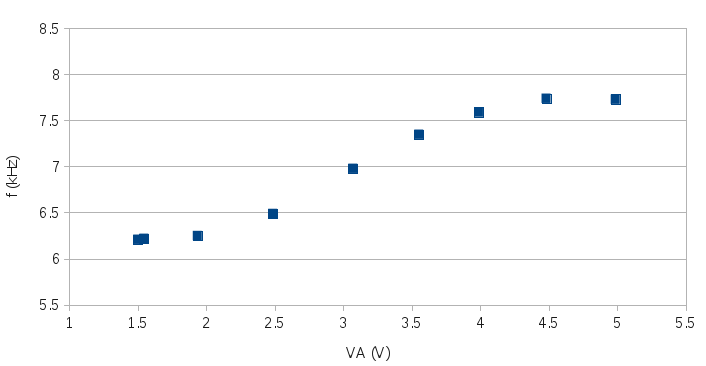
\includegraphics[width=0.45\textwidth]{./pics/vco_2.png}
	\caption{ Gráfica de frecuencia de salida $f$ vs. tensión de entrada $V_A$ para $R_1$=4.7 k$\Omega$ y $C_x$=10 nF.}
	
	\label{vco_2}

\end{figure*}


\section{Análisis de resultados y conclusiones}
\subsection{Medidas de características DC de inversores NMOS.}
En esta parte de la práctica se observan algunas fallas en las mediciones, que se ven en lo siguiente: 

\begin{itemize}
	\item El valor de $k_n$ tiene una desviación estándar grande, que es comparable al valor experimental dado (promedio de los datos).  
	\item La tensión de umbral fue diferente cuando $R_D=1$ k $\Omega$. 
\end{itemize}

Esto se atribuye principalmente al ruido visto en la señal, como se ve en la figura~\ref{p1ff22}, lo cual hace que al hallar las parejas $V_{in}$, $V_{out}$ se tengan lecturas inexactas.

De igual modo, al comparar con el modelo de SPICE se tiene que el valor nominal es $k_n=0.111$ mA/V$^2$. Se tiene por tanto que el valor experimental se aleja considerablemente del valor nominal, siendo más del triple.
 
\subsection{Osciladores}
En el caso del oscilador de anillo, se tiene que la principal limitación es que dada una frecuencia de oscilación es difícil lograr una configuración que cumpla con dicha frecuencia, pues el circuito depende de los parámetros de tiempo de los transistores, que pueden variar notablemente respecto a los valores nominales. 

En el caso del VCO, se tiene como principal desventaja que la ganancia y la forma de onda obtenida a la salida es muy sensible a la variación de la tensión de entrada. Sin embargo, es sencillo obtener una frecuencia específica de oscilación variando la tensión de entrada y los valores de $R_1$ y $C_x$.



\bibliographystyle{ieeetran}
\begin{thebibliography}{99}


  \bibitem{it1} CD4007 NMOS and PMOS transistor SPICE models. Disponible en \url{http://www.cs.uoi.gr/~tsiatouhas/DigElecIntro/CD4007.lib}.

\end{thebibliography}
\end{document}
